
\section{Derivable functions can be described in first-order logic}
\label{sec:to-logic}
We show in this section that derivable functions can be implemented by first-order transductions. We write $\voctype \rSigma$ for the vocabulary of a type $\rSigma$ as given in Definition~\ref{def:type-model}.

\begin{proposition}\label{prop:to-logic} If $f : \rSigma \to \rGamma$ can be derived from the atomic functions using combinators, then there is a first-order transduction $g$ 
    which makes the following diagram commute
    \begin{align*}
        \xymatrix@C=3cm{
            \rSigma \ar[d]_{a \mapsto \underline a}\ar[r]^f &  \rGamma \ar[d]^{a \mapsto \underline a} \\
            \text{relational structures over $\voctype \rSigma$} \ar[r]_g &  \text{relational structures over $\voctype \rGamma$}.
        } 
    \end{align*}    
\end{proposition}
    
    \begin{proof}
    The proof is by induction, following the definition of derivable functions. The proof is easy, and consists mainly unfolding of the definition. We will treat only the cases of $\unit_\rSigma$ and $\flatt_\rSigma$ to illustrate this process.
    
    In the following, it will be convenient to use, as part of the vocabulary of $\rSigma$, the unary relation  $\mathsf{Port}_\rSigma$ which selects the ports of the structures over $\voctype\rSigma$; and the binary relation $\sqsubset_\rSigma$ which orders these ports. By induction on $\rSigma$, we can show that both relations are definable by first-order formulas over  $\voctype \rSigma$.
    
    \begin{enumerate}
    \item $\unit_\rSigma$. Given an element $x$ of $\Sigma$, let us show how the fucntion $\unit_\rSigma(x)$ can be implemented using an fo transduction.  The copying constant is 2,
    the first copy will contain the whole structure $\underline{x}$ and the second copy will select only the ports of $\underline{x}$ which will serve as the ports of the structure $\underline{\unit_\rSigma(x)}$ (see Figure~\ref{fig:transductionUnit}).  The universe formulas are then:
    \begin{align*}
    \varphi_1(x)=\mathsf{True} \qquad \varphi_2(x)=\mathsf{Port}_\rSigma(x)
    \end{align*}
    \begin{figure}
    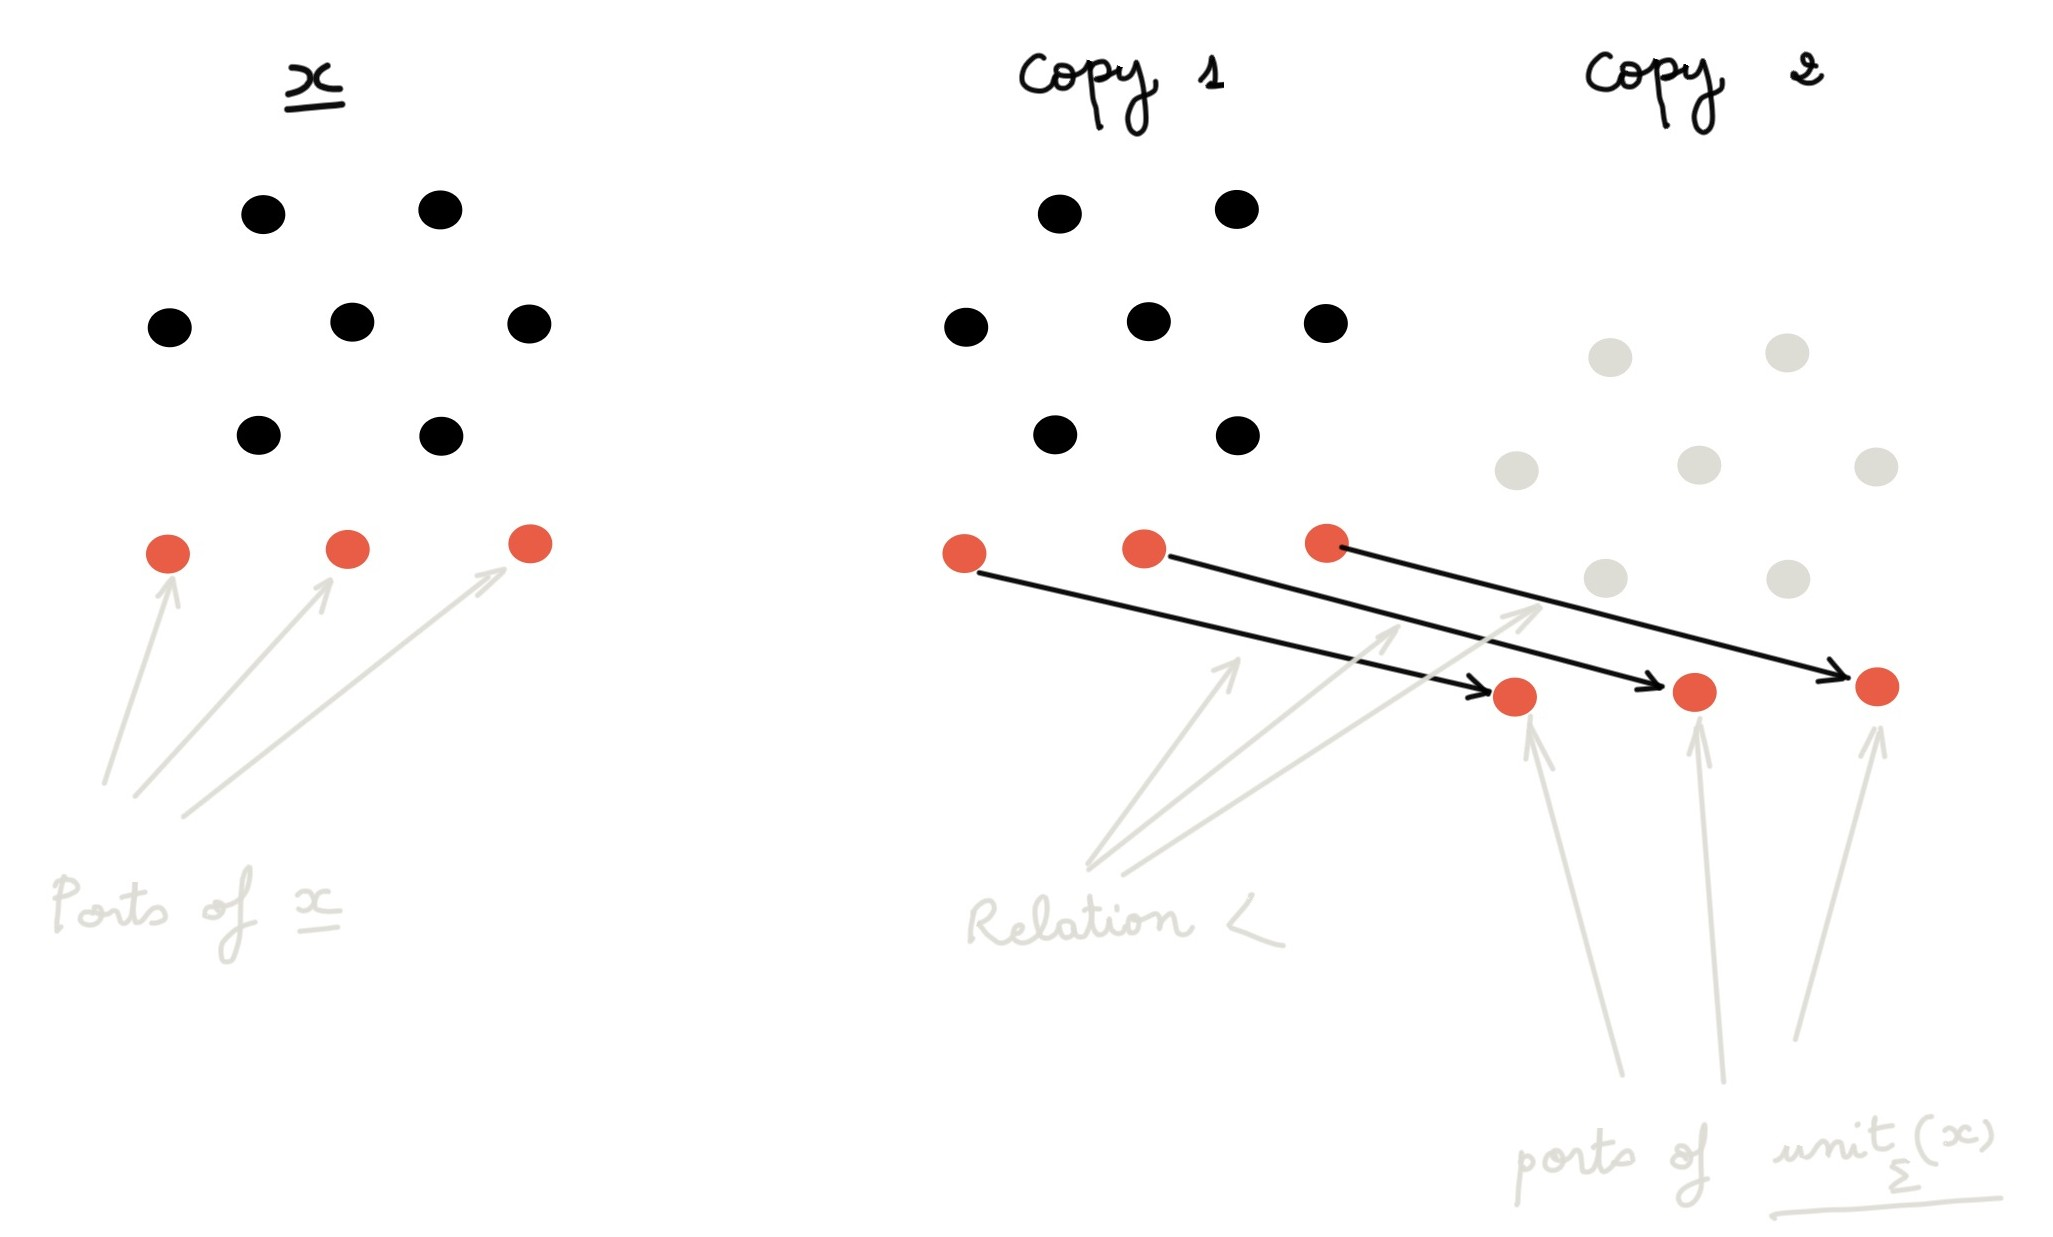
\includegraphics[scale=.1]{MyPic8.jpg}
    \caption{}\label{fig:transductionUnit}
    \end{figure}
    In the first copy, the vocabulary of $\rSigma$ will be interpreted as in the original structure, and as the empty set in the second copy. That is, for every unary relation $R\in \voctype \rSigma$ and for every binary relation $S \in \voctype \rSigma$, we set:
    \begin{align*}
   \varphi_R^{1}(x)=R(x) \quad&\quad \varphi_S^{1,1}(x,y)=S(x,y)\\
   \varphi_R^{2}(x)=\mathsf{False} \quad&\quad \varphi_S^{2,2}(x,y)=\mathsf{False}
\end{align*}      
Let us interpret the relations $<$ and $\sqsubset$ of $\voctype \tmonad\rSigma$. The  ports of $\underline{\unit_\rSigma(x)}$ inherit the order of the ports of $\underline{x}$, this is why we set:
\begin{align*}
\varphi_\sqsubset^{2,2}(x,y)=x\sqsubset_\rSigma y
\end{align*}
The descendent relation $<$ connects the $i^{th}$ port of $\underline{x}$ to the $i^{th}$ port of $\underline{\unit_\rSigma(x)}$. Since these nodes come from the same node in the original structure, we set:
\begin{align*}
\varphi_<^{1,2}(x,y)=x=y
\end{align*}
 \item {$\flatt_\rSigma$}. Let us consider now the function $\flatt_\rSigma$ and let $t$ be an element of $\tmonad\tmonad\rSigma$. 
 
Notice first that the input vocabulary $\tmonad\tmonad\rSigma$ contains two layers: the first is the vocabulary of $\tmonad \rSigma$, which describes the struture of the nodes of $t$. It contains in particular a descendant relation, which we will denote by $<_\rSigma$ and a port orderings which we will denote by $\sqsubset_\rSigma$. The second layer describes the top-level structure of $t$: it contains a descendant relation which we denote by $<_{\tmonad\tmonad\rSigma}$ and a port ordering which we denote by $\sqsubset_{\tmonad\tmonad\rSigma}$.

 To implement the flattening function, we need only one copy of the original structure. The universe will contain all the elements of $\underline{t}$ except the inner ports, that is the ports of the structures $\underline{t(x)}$, where $x$ is a node of $t$.    
 \begin{align*}
 \varphi_1(x)=\neg \mathsf{Port}_{\tmonad \rSigma}(x)
 \end{align*}
The relations of the vocabulary of $\rSigma$ are interpreted as in the original structure. The ports of $\underline{\flatt_\rSigma(t)}$ are the ports of $\underline{t}$ and their ordering is the same, meaning that
\begin{align*}
\varphi^{1,1}_{\sqsubset}(x,y)= x\sqsubset y
\end{align*}
Let us interpret the descendent relation $<$.  If $m, n$ are nodes of the structure $\underline{\flatt_\rSigma(t)}$, then $m$ can be a descendant of $n$ for the relation $<$ for two reasons:
\begin{itemize}
\item Either $m$ and $n$ come from the same node $x$ of $t$, and $m$ is a descendant of $n$ in $\underline{t(x)}$ for the relation $\tmonad \rSigma$,
\item Or $n$ and $m$ come from two distinct nodes of $t$, call them $x$ and $y$ respectively. In this case, the node $y$ is a descendant of $x$ in $t$, and there is a port $o$ of $\underline{t(x)}$ such that $n\leq_{\tmonad \rSigma} o$ and $o<_{\tmonad\tmonad \rSigma} m$.  
 \end{itemize}
These situations are illustrated in Figure~\ref{fig:transductionFlat}. Thus, the formula describing the relation $<$ for the struture of $\flatt_\rSigma(t)$ is:
\begin{align*}
\varphi^{1,1}_<(x,y)= x<_{\tmonad\tmonad \rSigma}y \vee \exists z\ \ \ (x<_{\tmonad \rSigma}z \wedge z<_{\tmonad\tmonad \rSigma} y) 
\end{align*}
    \begin{figure}
    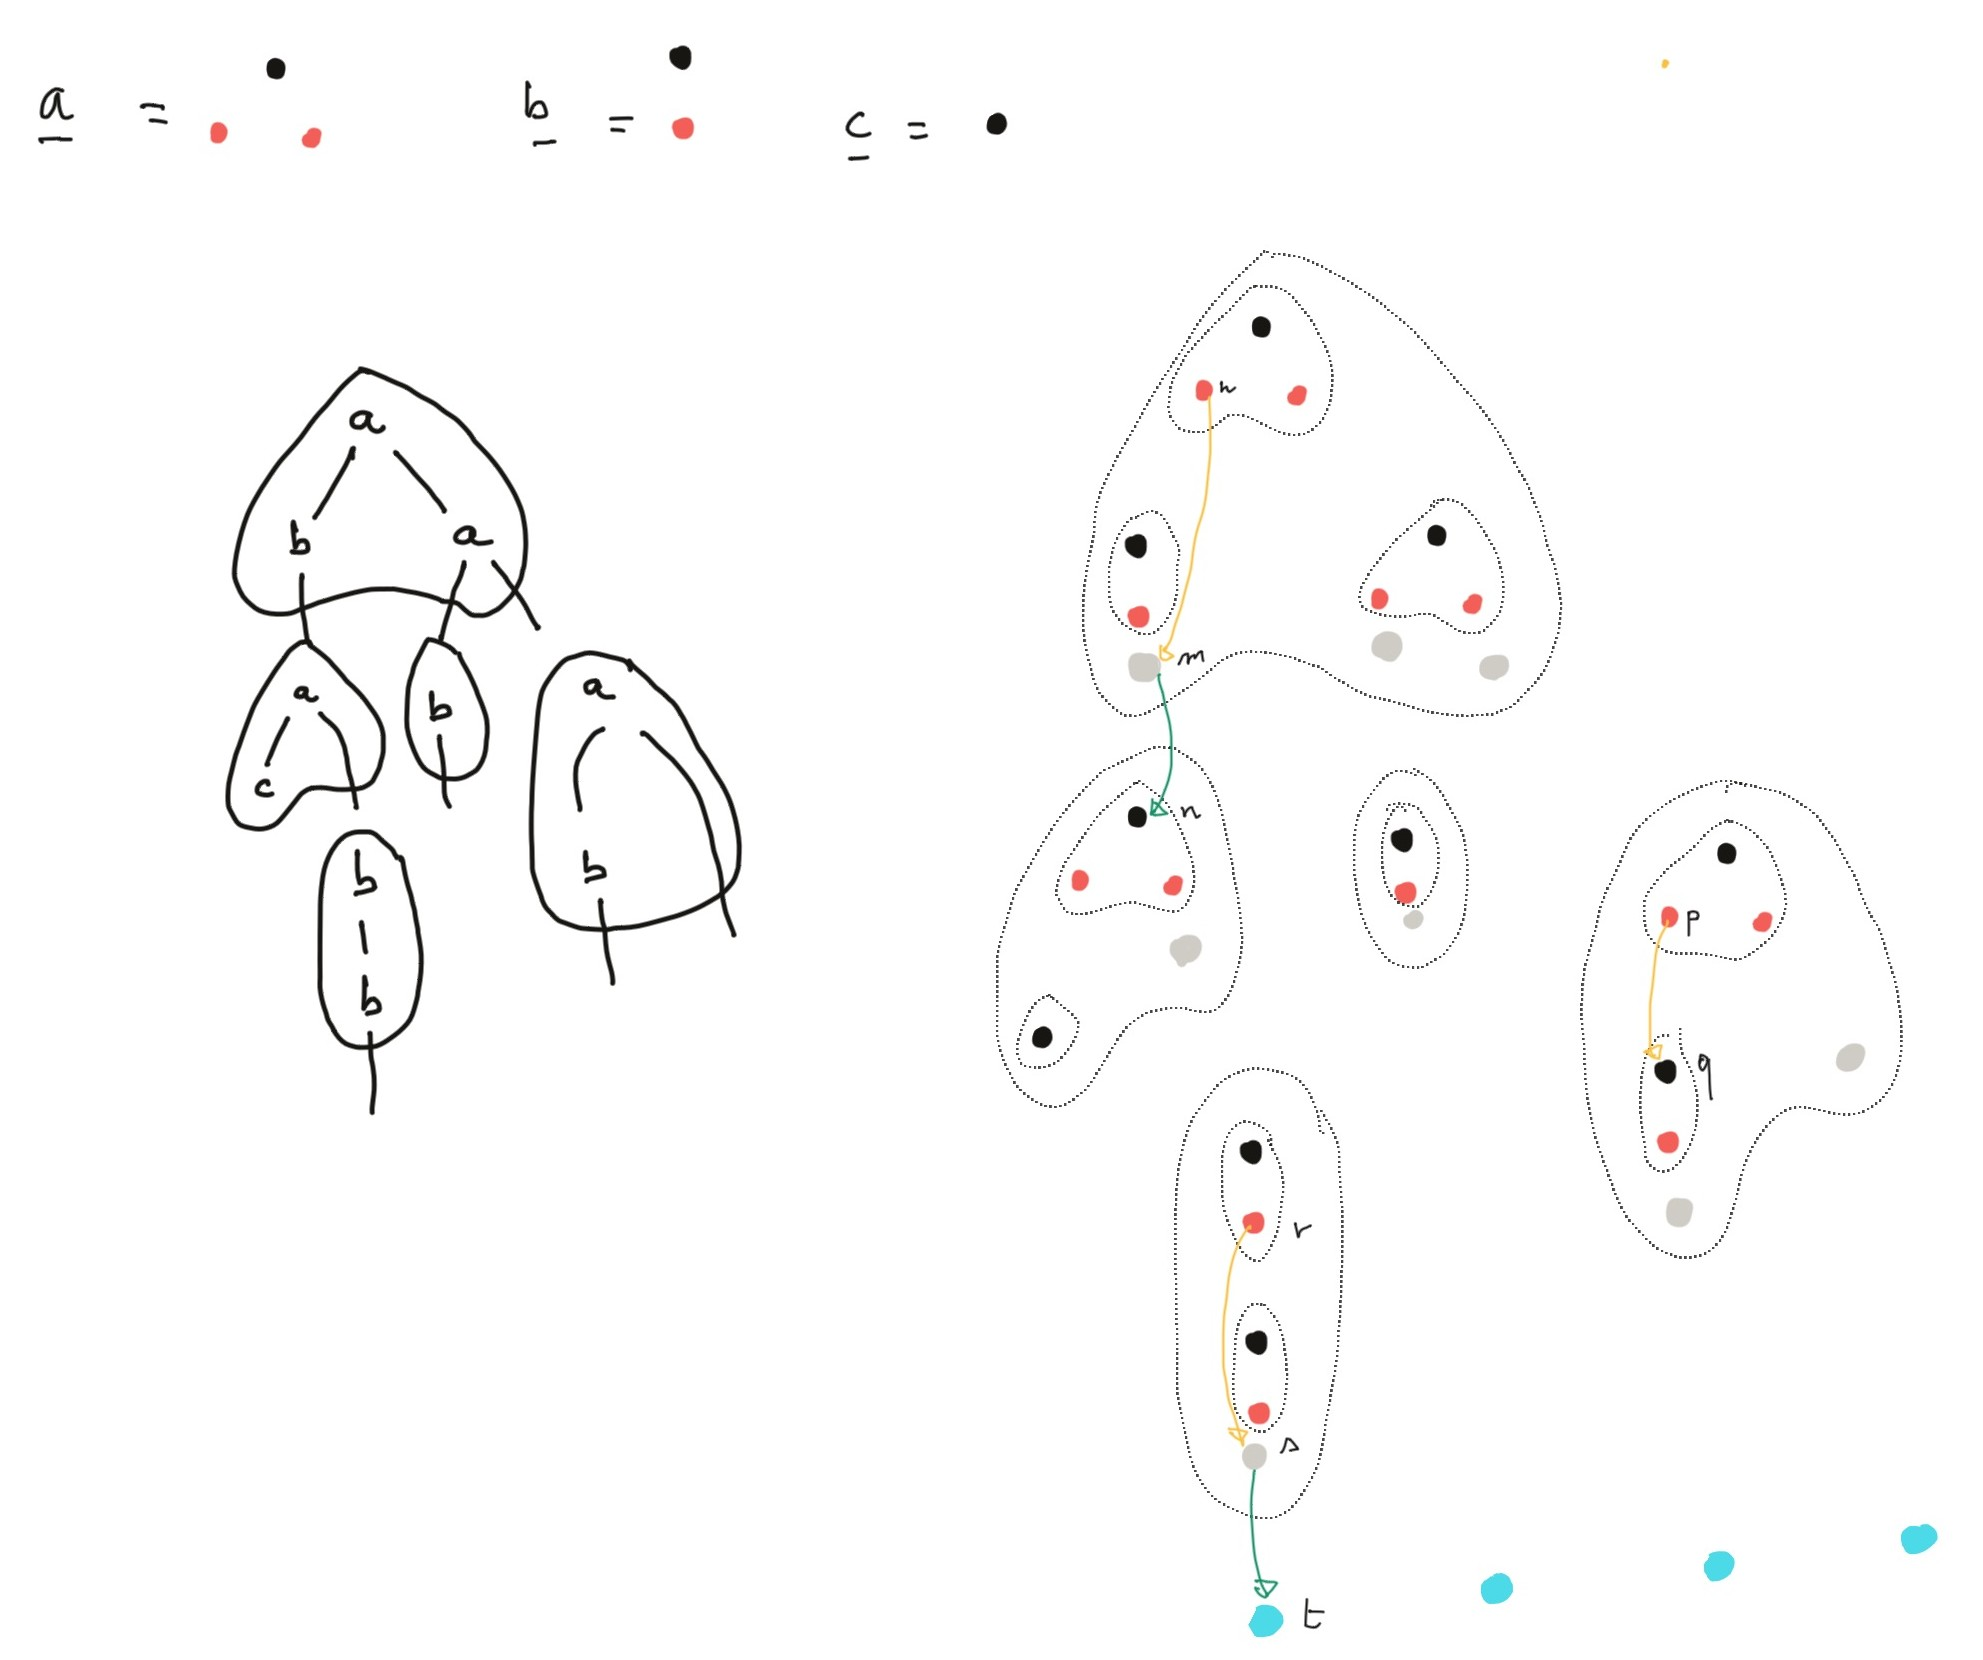
\includegraphics[scale=.1]{MyPic9.jpg}
    \caption{}\label{fig:transductionFlat}
    \end{figure}
%\item $\ranked{\unfold}_k$. Let us consider now the function   $\ranked{\unfold_k}$. For the sake of readability, we will consider here only the case where $k=2$.
%Recall that 
%\newcommand{\voc}[1]{\mathrm{voc}#1}
%\begin{align*}
%\text{Input vocabulary} \qquad& \ranked{\voctype(\tmonad  \reduce 2 (\Sigma \otimes \Sigma))} := \color{blue}{\voc \Sigma} + \color{green}{\voc \Sigma}  \color{black}{+ \rightarrow + < + \sqsubset}\\
%\text{Output vocabulay} \qquad&
%\ranked{\voctype(\reduce 2 (\tmonad\Sigma \otimes \tmonad  \Sigma))} := \color{blue}{\voc \Sigma} \color{black}{+} \color{blue}{<} \color{black}{+}\color{blue}{\sqsubset} \color{black}{+} \color{green}{\voc \Sigma} \color{black}{+} \color{green}{<} \color{black}{+}\color{green}{\sqsubset}  \color{black}{+ \rightarrow}
%\end{align*} 
%Let $a$ be un element of $\ranked{\tmonad  \reduce 2 (\Sigma \otimes \Sigma)}$. We will explain how
% $\underline{\unfold(a)}$ can be obtained from $\underline{a}$ via a first-order transduction. 
%\begin{itemize}
%\item The universe.  We will need two copies of $\underline{a}$. 
%In the first copy, we keep all the nodes except the (intermediary) $\ranked {\reduce 2 (\rSigma \otimes \rSigma)}$ ports. In the second copy, we keep only the $\rSigma$ ports which are "directly" connected to the ports of the structure $\underline{a}$.    
%\begin{align*}
%\varphi_1(x)=& \neg \mathsf{port}_{\ranked {\reduce 2 (\rSigma \otimes \rSigma)}}(x) \\
%\varphi_2(x)= &\mathsf{port}_{\color{blue}{\Sigma}}(x) \vee \mathsf{port}_{\color{green}{\Sigma}}(x) \wedge ( \exists y\  \ x \rightarrow y\ \wedge\ z=\mathsf{succ_<}(y)\ \wedge\ \mathsf{port}_{\ranked{\tmonad \reduce 2 (\Sigma \otimes \Sigma)}}(z) )
%\end{align*}
%\item Interpretation of the vacabularies $\color{blue}{\Sigma}$ and $\color{green}{\Sigma}$. In the first copy, the interpretation of these vacabularies is exactly the same as in the original structure. In the second copy 
%\end{itemize} 
\end{enumerate}
           \end{proof}
   Let $E$ be a totaly ordered set. We set $\mathsf{Mon}^E$ to be the monoid whose ground set is 
   \begin{align*}
   \{f:E\to E \ | f \text{ is monotonic}\}
\end{align*}    

and whose multiplication is functions composition.  The elements of $\mathsf{Mon}^E$ can be represented graphically as:
     

We show that the monoid $\mathsf{Mon}^E$ is aperiodic.
     \begin{proposition}\label{prop:MonIsFo}
The monoid $\mathsf{Mon}^E$ is aperiodic.     
     \end{proposition}
     
     \begin{proof}
     Let $f$ be an element of $\mathsf{Mon}^E$. We define \emph {its graph} as the directed graph whose set of vertices is $E$, and which contains an edge $i\rightarrow j$ if $f(i)=j$. Note that the out-degree of the nodes is 1. To show Proposition~\ref{prop:MonIsFo}, we start by extracting some properties of these graphs.
     
The first one is that the weakly connected components of these graphs are intervals. With this property, we can treat only the graphs with only one weakly connected component, since those are independent. 
     \begin{lemma}
     If $f$ is an element of $\mathsf{Mon}^E$ and $I\subseteq E$ is a weakly connected component of the graph of $f$, then $I$ is an interval. 
     \end{lemma}
     
     \begin{lemma}
     If $f$ is an element of $\mathsf{Mon}^E$ whose graph $G$ is weakly connected, then 
\begin{itemize}
\item there is a node $n$  having a self loop in $G$,
\item there is a directed path from any node of $G$ to $n$. 
\end{itemize}     
 We call $n$ the \emph{attractor} of $f$.    
     \end{lemma}  
     The attractor is unique. Indeed if we had two attractors $m$ and $n$, we would have a directed path from $m$ to $n$. And since $m$ has a self loop, its out-degree would be at least 2 which is not possible. 
      
    \begin{lemma}
    Let $f$ be an element of $\mathsf{Mon}^E$.  If there is a directed path of lenght $p$ from $m$ to $n$ in the graph of $f$, then there is a directed path of lenght $1$ from $m$ to $n$ in the graph of $f^p$.
    \end{lemma}
     \end{proof}